%===================================== CHAP 5 =================================

\chapter{Discussion} \label{cha:discussion}
This chapter discuss the questions on the research question, and discuss the results. Using knowledge from both the litterature review and the case study. This discussion will give the foundation for the conclusion and further work discussed in chapter \ref{cha:conclusion}.

This research tries to understand how the Norwegian Construction Industry can perform better in terms of labor productivity through the use of Agile processes and Digital transformation. The research is not to measure productivity, rather identify essential instruments for the rest of the industry to take into use. The results indicate that the use of Lean and groupware requires a change in project setup, moreover, challenge in low utilization if not appropriately managed. This challenge is identified in the LSB-project in the interaction between the workers, where a lack of basic methodology understanding and overlapping software utilization are the critical impact on the project's utilization of the digital and methodological potential. 

This result suggests the how does the project realize the potential of Lean methodologies and the applied digital tools. This chapter will discuss this result around the three principal subjects. First, as reviewed in chapter \ref{chp:litterature}, constructing a complex construction is making people interact, coordinate and comunicate. Furthermore, a effective methodology will suit project management. Moreover, the interviews revield huge digital potential, in which the project can benefint. Thus, the three subjects are cooperation and interaction, methodology, and digital potential. Also, the chapter will discuss at different approaches defeating these challenges.

\section{Cooperation and interaction}
Introducing cooperation in the CI implies some introduction of legal papers and contracts. How these contracts influence interaction in the project vary with every contract. Some managers tend to what is known as "contract managing" – making the contract dictate the management. Also, prior interaction between actors is quintessential for cooperation for a new project \cite{rolfsen}. However, for a project to work, communication and knowledge sharing is vital in project cooperation. 

\subsection{Contracts and legal issues}
Managing a large scale construction project, or a large scale project in general, will introduce some contracts. With a good foundation based on reliable contracts, the project is arguable on the right track, on the legal side, that is, although there is still one barrier in the Norwegian CI. That is the period between the programming and the design phase in the project lifecycle, described in section \ref{sec:CI_context}. This period of waiting from programming is done, to the design phase can begin, makes for a substantial change in the project's actors. Thus, much of the potential knowledge is lost. 

The LSB-project makes use of a customized contract, named \textit{Totalentreprise med forutgående samspill}. The implications of a new contract have shown to be a more complicated issue than the intention. The difference is the level the contract dictates the management and interactions. Prior interaction contracts are proven to improve cooperative behavior in a project \cite{wang2017prior}. Thus, the legal barriers can not be of blame in the LSB-project. The intention of the contract was for the contract to support the interaction and prevent errors in the design. Also, considering the project consist of about 30 different contracting firms. The result is a problem in harmonization between the actors, thus leads to difficulty utilization of lean \cite{miller2002harmonization}. In the interviews, on the other hand, the contractors explain they feel harmony in the design phase. Also, the harmonic sense is for the new contracting to blame. Usually, these issues do not come in the design phase. Therefore, the results of this can not say if the contract applied will aid the LSB-project. The indications from the contractors part in the design phase are, hence, promising. 
    
The project has clear role expectations, as Rolfsen promotes\cite{rolfsen}. The results show that even though the project has clear role expectations, it seems like the managers and PLs have problems in decision making. One might think that the contractors are up to secure their contracts and increase their revenue. However, based on prior research, one might argue that a more plausible explanation has to do with risk allocation \cite{zaghloul2003construction}.  Still, the problem is not the discussion, but failing to make a decision. This issue might be the case when applying LOD in the project. People are not familiar with this methodology, thus, not recognizing the use. 

The implications of the insecurity can lead to delays and reduced utilization of human resources, which again leads to low LP. Then again, taking the wrong decision and spending time fixing it will cause much greater damage. 

\subsection{Communication}
Cooperation and interaction heavily rely on sufficient communication, both direct and indirect communication. In both cases, the project is using digital tools, supporting communication. In the case of direct communication, face-to-face communication is to prefer. Email is the most used tool. So much, that it could be frustrating. Hence, the comment in figure \ref{tab:software-map}. Some teams have decided to use Microsoft Teams supporting direct messaging in chat. The problem of using separate digital tools, in each team, is the forming of silos. Where every discipline work well together, but the discussion with others has to happen in different settings and using other tools. This use is arguing for a common platform for discussion. 

Both Teams and Blink offers such a platform. The reports about Blink, as one can see in table \ref{tab:software-map}, implicates the functionality of the software is not understood. Moreover, several teams have chosen to use Teams. The challenge in using Teams is that the functionally in the direct messaging is supported in Blink, while the functionality of task management is supported in both Cogito and BIM 360. Moreover, both BIM 360 and BIMcollab offers much of the same functionality in BIM cooperation. The teams chose to supplement with the tools they need, more than making the best of the tools procured by the project. The challenge is for the project manager to procure software that is the best for the project, covering what they believe is the best for the project. Hence, the rules of procurement. The arguments for applying Teams are, as we can see in the software map \ref{tab:software-map}, mostly prior knowledge and use. Also, the manager did not intend to use and do not see the need for Blink to be a direct communication platform, even though the manager knows of the functionality. 

The time of procurement is proven to be essential in use. Both in the case of Blink and BIM 360, the design phase had been going on for quite some time. So, in the time where Teams and BIMcollab were taken in to use, there were no other tools to use, sustained by the manager.

Email is a commonly used groupware, also in the LSB-project. In a project with a large number of actors, as in the LSB-project, email can tend to be overused, and therefore, ineffective. The difference in email appreciation is, of course, present, as seen in the software map \ref{tab:software-map}. Hence, the different citations from participants in different roles of the project, where an Associate will appreciate using email much more than a Discipline Leader and a BIM Manager. Consequently, the project has chosen to procure other services supporting communication and, thus, also project management.

The challenge in procuring new tools is having the user take them into use; hence, Blink and BIM 360. The "critical mass"-problem \cite{markus1987toward} is seen in the project, for example, in the use of Blink. On the other hand, when looking at Cogito, where almost everyone is present, the tool is not overly used; thus, one can not perceive the critical-mass problem. Also, how the project is using Cogito is mostly based on face-to-face interaction, supported by the tool. This phenomenon is present in figure \ref{fig:cogito_use}, showing a drop in use before and after the Covid-19 pandemic. This reduction in use was no surprise when presented to a representative from Statsbygg; thus, the use of Cogito is mostly not a part of the daily routine, rather, a part of a group exercise. This fact supported in two distinct comments about the case. First, the Associate about not checking Cogito, before everything else on the agenda, is done. Second, the Engineering Manager's quote about the use of Cogito in meetings. 

The barrier utilizing Cogito aligns with Grudin \cite{grudin1989groupware}, where the tool changes the way of working. Moreover, the tool does not give equal benefits to users. Also, when not being used too often, the effect is multiplied. Moreover, SharePoint, Teams, BIM 360, and BIM collab all share the same feature of task management. Additionally, a BIM Coordinator argues for SharePoint to replace Cogito.

\begin{figure}
    \centering

    \caption{Illustration of Cogito use before and after lockdown, shown as CPU use on the server.}
    \label{fig:cogito_use}
\end{figure}

Another reason for the lack of Cogito use is the issues mentioned by the participant. Most of the feedback was regarding the lack of overview. Contractors used to Gantt-diagram, and not Lean Construction, has a problem with not having the general overview. Hence, the tool needs to meet the requirement of the group \cite{subramanyam2010user}. Moreover, one can argue for different visibility in project progress, using burn-down-chart, often used in SCRUM \cite{sutherland}. Another issue reported is the lack of communication offered by the tool. The notification functionality does not work; thus, the tool does not communicate sufficiently with the users. 

Also, Interaxo received a large amount of negative feedback. The problem reported is useability issues and the difficulty in cooperating using the tool, as seen in \ref{tab:software-map}. The manager procured Interaxo, based on legal reasons. Constructing in Norway has to follow a certain level of documentation, using a tool qualified for use. The set of qualified tools is, unfortunately, small. Interaxo was best in class in the process of procurement. Moreover, the handling of documents often introduces interaction, and often, a team has to work together on a document; Making for an introduction of SharePoint or similar solutions. 

\section{Methodology}
The vision and strategies are an essential aspect of the management of the organization. The results contradict the claims of Buvik and Rolfsen \cite{rolfsen} that the development of a common philosophy: namely the vision, will aid the trust among team members. Arguably the "one project"-statement is helpful. What the participants have noted is the contract. Also worth noticing is that the project is still in the design phase, where the cooperation is quite harmonic in most projects. The problem in the LSB-project is that the top-down approach heavily influences the management. Thus, giving workers with little perception of the common philosophy. Furthermore, early and clear role expectations and early development of trust are problematic in a project where there is a high degree of turnover. The turnover is exemplified in the interviews, where one of the participants was the fourth to fill the role since the start in early 2018.
     
The top-down approach makes for a problematic implementation of a common philosophy, but also the implementation of lean. One of the principles of the agile manifesto \cite{agile_manifesto} states:
\begin{quote}
    \textit{Build projects around motivated individuals. Give them the environment and support they need, and trust them to get the job done.}
\end{quote}
    
One can argue that this statement is contrary to the approach used in the project. The managers have set a set of processes and ways of work, making the project utilize Lean on their command.  On the other hand, as we have seen in the results, most of the project workers do not know lean, thus, expect them to work in an agile matter without the support from the governing organization is absurd. Moreover, \textit{giving them the environment and support} is precisely what the manager has done when: (a) Implementing the sort of contracts eliminating potential conflicts and, thus, waste; (b) Utilizing Cogito making for early discovery of faults and avoid miss production; (c) Implementing LOD in the entirety of the project, also planning a "flow" process in the construction, using trains and wagons; (d) Making use of LOD offers a "just in time" production and unnecessary decisions to be made; (e) Working alongside the customer throughout the whole construction lifecycle, and with the implementation of Automatic Completion making sure a perfect result is achieved. 

All the actions (a-e) giving the right environment and support is ultimately a complete implementation of Aziz's five principles of Lean Methodology \cite{aziz2013applying}: (1) value, (2) value stream, (3) flow, (4) pull, and (5) perfection. 

This implementation leads to a tendency that the workers are working in the same way as done before. One can argue that the reason for the way of working is lack of practice, hence the lack of fundamental methodological knowledge. The project does not work as previously; hence, the aforementioned actions. This observation contradicts the claims from Ingvaldsen and Rolsen that the introduction of Lean can hamper the Norwegian working model \cite{ingvaldsen2012lean}. On the other hand, Ingvaldsen's argument is more valid in the construction process, where trains and wagons promote repetitive work.

The top-down approach reinforces the challenge of people not knowing the basics in Lean Construction. Most of the actions applied are also beneficial in a project not utilizing Lean; thus, the actors not recognizing the actions made to be Lean. This preception makes the actors seek old managing tools. The use of Gantt-chart is a prime example of this issue. The managers need an overview, more than the process control, supported by Cogito. There is no defined way of looking at the progress in Lean design. Thus, the need for using Gantt is obvious. Also, using Gantt in the planning of the construction process is required due to legal constraints. 

The project uses PPC to identify project progress. The PPC will only give progress as opposed to a predefined baseline, given by the initial planning. Thus, as long as the Gantt chart works as a baseline, it will serve as useful. On the other hand, Sutherland argues that Gantt-chart is always wrong \cite{sutherland}; thus, using something that is known to be wrong as a baseline is futile.

The project is using LOD in the entirety of the project, not only MMI in the BIM modeling. This approach is quite unconventional, not known for the workers. Let alone tricky for the workers not known to any LOD process beforehand. The underneath quote is an example of this issue. 

\begin{quote}
    \textit{"We do everything differently in this project. It is hard to plan for these levels of MMI"} \\
    - Ass. Project Group Leader
\end{quote}

LOD being essential in the pull and the flow of the Lean implementation makes for an important part for the workers to understand. Even though the workers do understand MMI and LOD, it does not seem like they understand how this correlates with Lean. This quote, underneath, being not entirely correct is an indication of the lack of knowledge of the total image. 

\begin{quote}
    \textit{"That is our way of answering to the Lean Principles in the project, I think"} \\
    - Ass. Project Group Leader, about using MMI
\end{quote}

Besides, LOD is not the only part difficult for workers to understand. As mentioned in the results, some do not know of Lean Design or believe Lean is something put into action come constructing. The project does have a problem with speaking out the actions taken regarding Lean, as seen below. This quote indicates workers not seeing the actions (a through e listed above) taken in the design phase.

\begin{quote}
    \textit{"...everything else. There is much more than just trains and wagons, which I have seen all but nothing of."} \\
    - Associate, about Lean in the project 
\end{quote}

The project, following the principals of Lean, is not bound to a way of writing task descriptions. As seen in the case, some inputs are more free text; this makes for a set of different ways of writing package descriptions. A challenge is the variety of tasks. Take, for example, the actions: some actions are a one-man-job, while others are clarifications between actors. Also, one has to consider the LOD in what to expect. 

There is no literature covering the writing of tasks, task naming, and task description in Lean Construction. The project uses natural language when writing task descriptions with no form of template or rules often makes for ambiguous tasks; the interpretation of the task can prove to be different. Moreover, problems reported corresponds with the requirements quality metrics, defined in table \ref{tab:requirement_quality}. Hence, a project utilizing Lean has to define a way of writing proper task descriptions. Being Lean implies minimizing waste. Writing proper requirements is, thus, an aspect of waste not covered by the project structure.

Looking at other industries implementing agile, such as Software development, Requirement Engineering (RE), is a complicated but essential process in design. Having a well-established RE-process makes for even better requirements \cite{pandey2010effective}. Moreover, writing high-quality requirements will ensure unambiguity and verifiable requirements \cite{carson2015implementing}. The International Council on Systems Engineering (INCOSE) proposes a set of standards for developing and evaluating sound requirements \cite{incose2015guide}. A subset of these are represented in table \ref{tab:requirement_quality}. Guided natural language \cite{rolland1992natural} and boilerplates \cite{daramola2012pattern} are different approaches achieving sound requirements.

\begin{table}
    \begin{tabular}{@{}lp{9cm}}
    \toprule
    \textbf{Type}       & \textbf{Description}                                                                                                         \\ \midrule
    Ambiguity           & The requirement contains terms or statements that can be interpreted in different ways.                                      \\
    Inconsistency       & The requirement item is not compatible with other requirement.\\
    Forward referencing & Requirement items make use of a domain feature that is not yet defined.                                                      \\
    Opacity             & A requirement item where rationale or dependencies are hidden.                                                               \\
    Noise               & A requirement that yields no information on problem world features.                                                          \\
    Completeness        & The needs of a prescribed system are fully covered by requirement items without any undesirable outcome.                     \\ \bottomrule
    \end{tabular}
    \caption{Verifiable requirements quality metrics \cite{incose2015guide}}
    \label{tab:requirement_quality}
\end{table}

The challenge in agile an agile process is the rapid change in requirements, thus, leading to another way of defining task descriptions—namely, the user stories used in Scrum \cite{sutherland}. User Stories will not directly work in a CI-project, but the idea of making a custom method for task descriptions is good. Also, a user story is often broken into the lesser task for the developers to deliver, because a User Story could include much work influencing the lode of workers \cite{liskin2014we}; Much like Milestones, Key-point, and deliveries, which are all broken down.

\section{Digital potential} \label{sec:digital_potential}
One of the most important pillars of the LSB-project is digitalization. Thus, the project has high expectations for digital utilization. The major digital initiative the project has done is the use of 3D modeling and the use of BIM. Several interviewees mention BIM as an essential aspect of interaction. 

\textit{"Using BIM gives an exceptionally effect. This is the future of the construction business. ...It becomes very conceptual. Therefore, easier to understand a problem."} \\
– Discipline Leader, about BIM

The design of the project started with PG, using a local server storing the BIM-files, designing the project. When the project started growing, the problem of using this local server occur. Issues with downtime and access caused the project to move, from a stationary server to a Cloud-based service run by Azure. Once every week a responsible, in every discipline, does export of the work done. The export, from every discipline, is then put together to enrich the model in Azure. Using the cloud-based system has been a powerful enhancement to the productivity of the project, and is noticed by the project staff. 

Some of the disciplines, including the architects, have set up automatic exportation of the files. Though, commit the exportation on a private computer. At times the responsible forget this, then closes the computer, forcing the automatic export to quit. The disciplines who have not set up an automatic export do this manually. Which takes time - up to two hours evety time, also the responsible can forget about it. The exportation used to take place once every two weeks, but when the interviews took place, the every week iteration had started. Also, talks of twice a week was inititiated. If the exportation should take place twice a week, a person responsible has to sit and wait through the exportation for up to four hours a week!

The project has a lot to gain using automatic export throughout the project, in every discipline. Hence, the move to a cloud-based system and how this impacts the working environment. Several responsible have expressed a need for a computer, handling the automatic export stationary in the project office. 

There is much potential in digitalization and automation of the BIM- and modeling-loop. The project wastes considerable time exporting and uploading files to different platforms, depending on the recipient. Moreover, several interviewees report of having a central computer for automatic export would be beneficial, which will be time-reducing for the one responsible for the export. Though, no one talks about a 100\% cloud-based system, where one can extract export from the sum. 

Such a system is described, by Chuang \cite{chuang2011applying}, with a Software-as-a-Service (SaaS) cloud-architecture. This way gives the user access to both manipulate and visualize the model from where ever. Moreover, the solution promotes communication and decrease silo-structure. A challenge Chuang discuss is the need for an excellent user interface (UI) and usability. BIM 360, already procured by the project, could eventually do this. For the project, BIM 360 suits as a web portal for others to see the modal, more than an actual design tool, furthermore tools previously used are still in use. Thus, the need for a design tool is not essential when they can use Revit and ArchiCad. Also, the contractors can decide which tool they want to use, thus, changing to a new tool is problematic. One argument is the usability of the new tool, but also, the contractors do pay for using their tools, thus changing to another will be costly. Moreover, learning to use a new modeling tool will be challenging; hence, the need for a quality UI. A different challenge in applying the Cloud-BIM system is all the plugins and supporting software used to create the model. These tools are still not cloud-based.

Another vital initiative is the use of Cogito. Taking the risk of totally new software could cause some issues underway. Sure, not everything has been a bed of roses. The project has cooperated with the supplier, improving the software according to the feedback from the user. There is even a page within the software where the users can give feedback directly to the developers and see the progress of their issue, seen in figure \ref{fig:cogito_feedback}. Despite the possibility of feedback, several of the participants reported issues with the software. A repeating factor was the lack of communication within the software. 

\begin{figure}
    \centering
    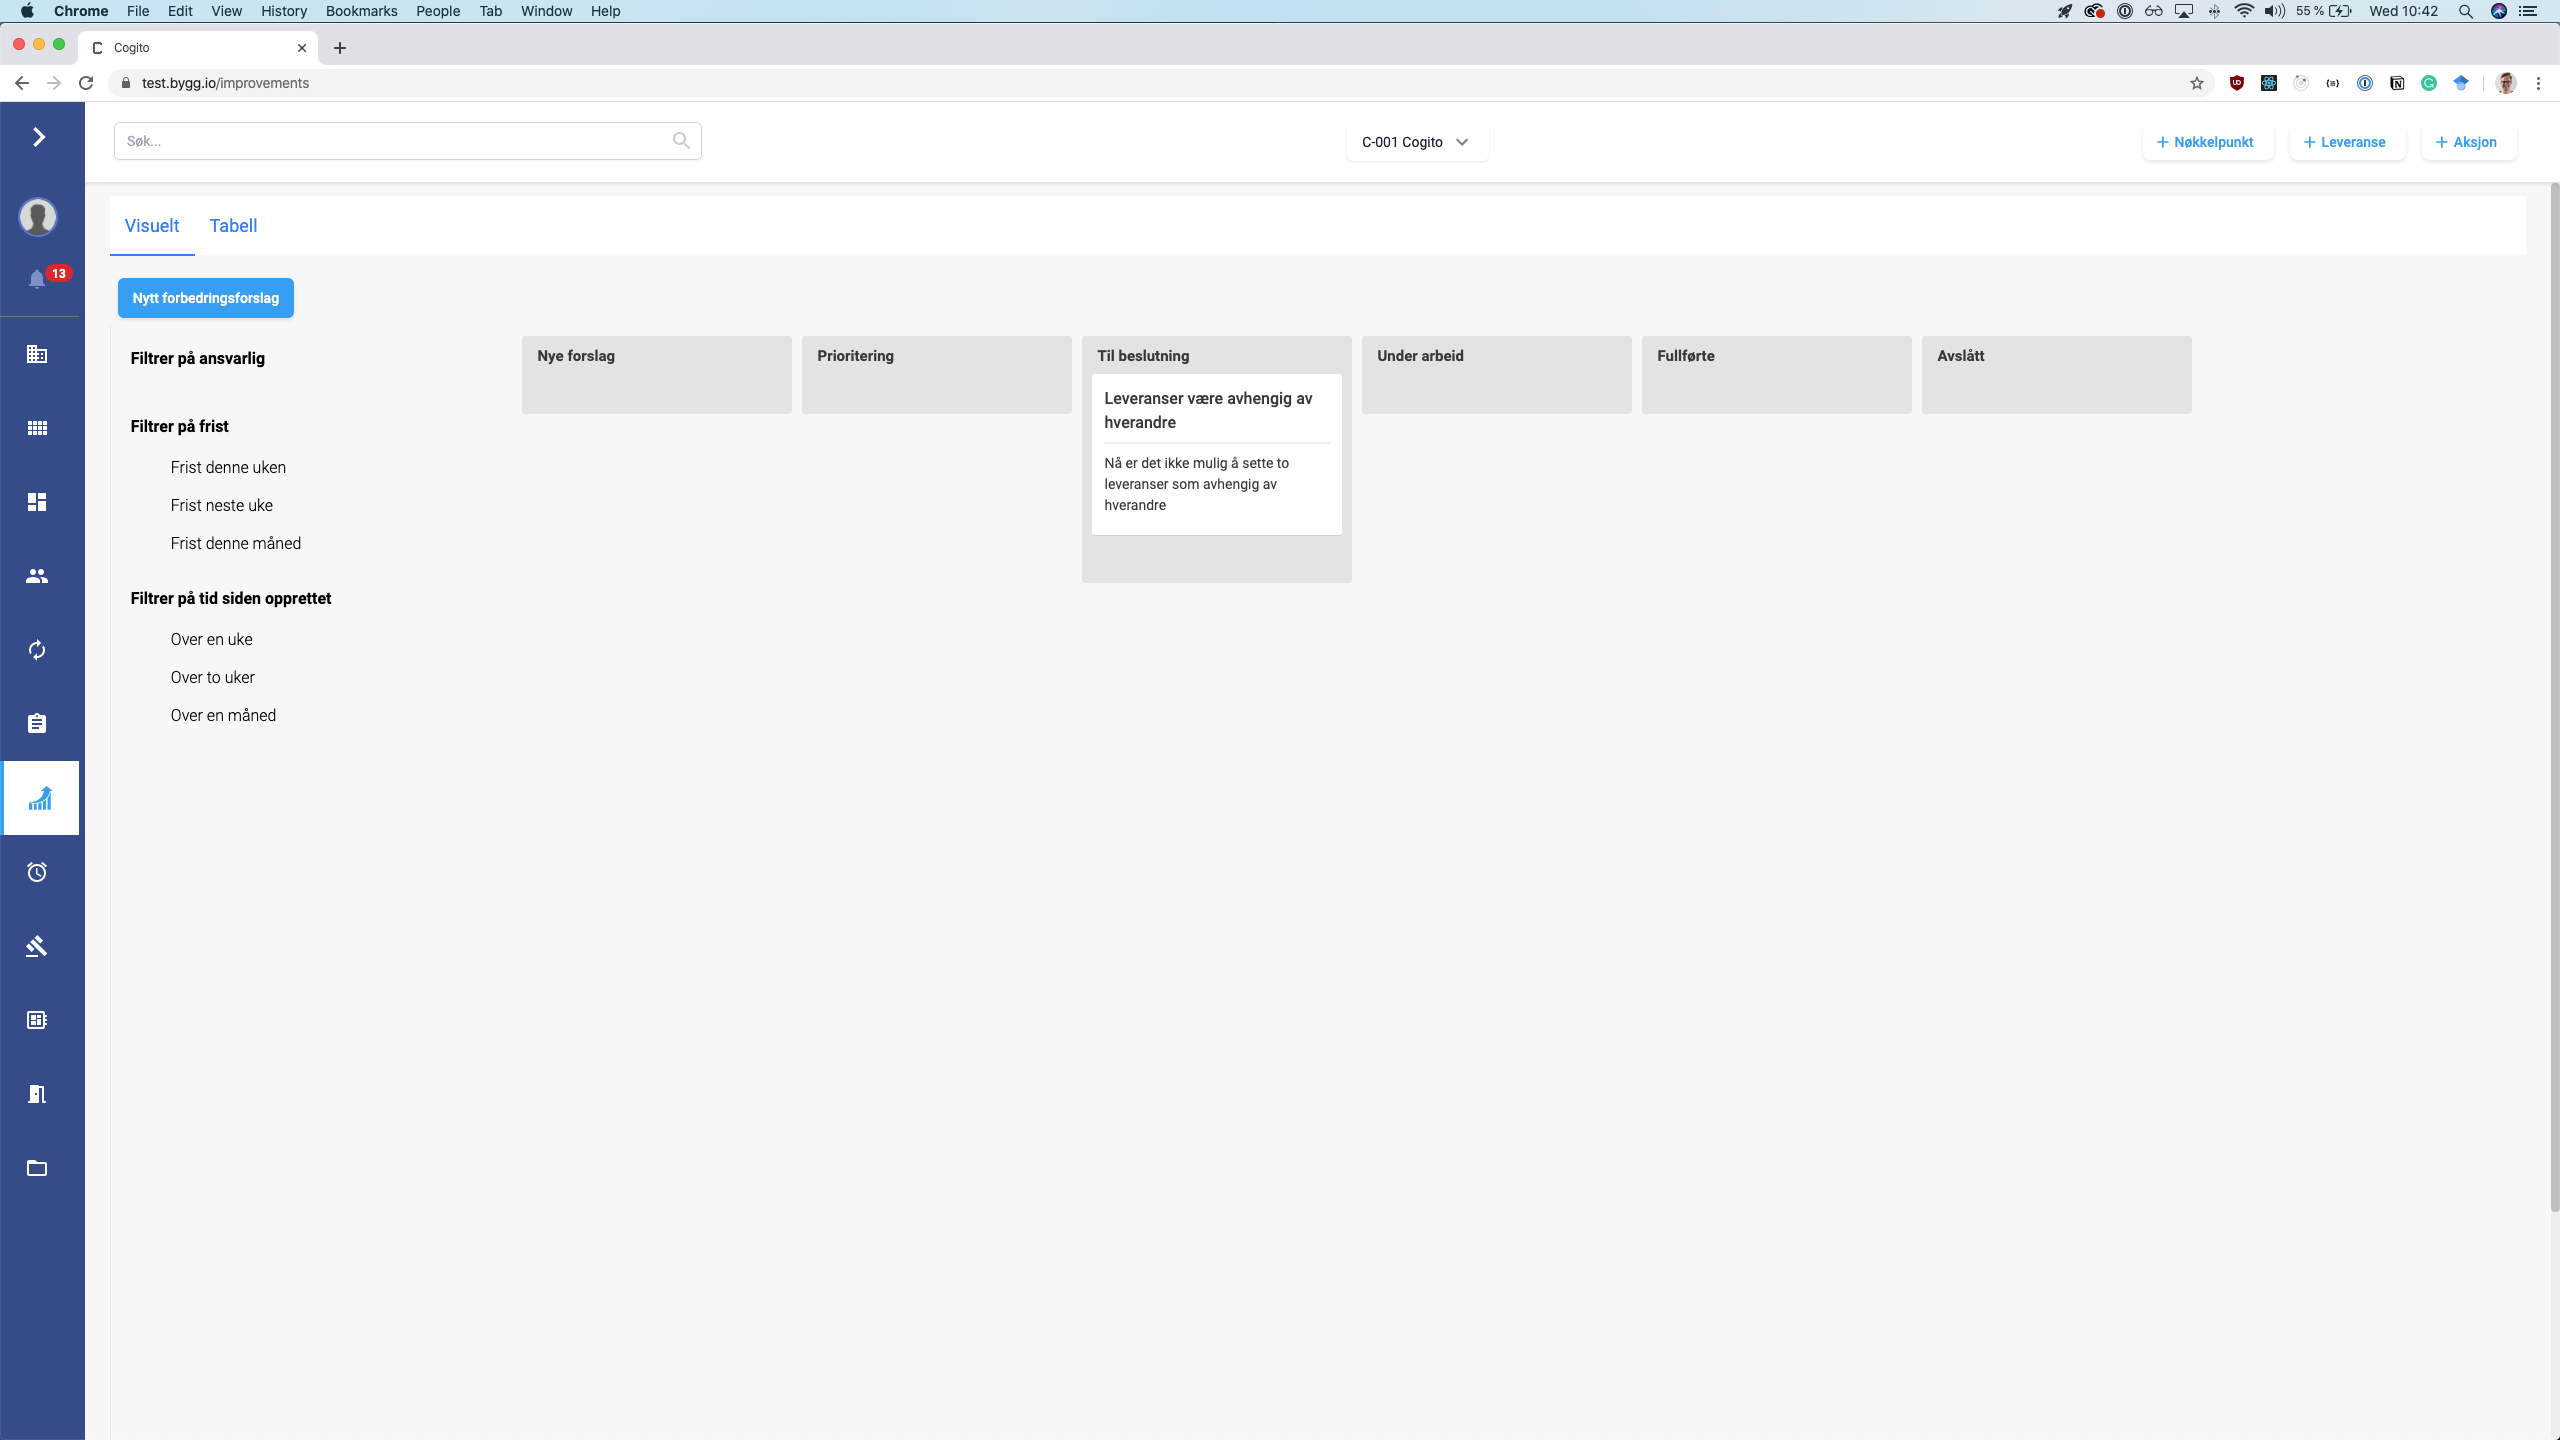
\includegraphics[width=\textwidth]{fig/cogitos_feedback.png}
    \caption{The feedback module in the Cogito tool. Serving as an continuous improvement of the tool for the project.}
    \label{fig:cogito_feedback}
\end{figure}

Introducing Cogito had the goal of reducing email, giving packages through the tool, rather than via email. PLs are writing packages into Cogito, but the notification is more often than not given orally, in meetings or over the desk, or via email. This Causing twice the work, rather than writing it directly into Cogito. As one can see in the two quotes below, an argument for communicating the package is for the inadequate notification in Cogito. Also, describing a package is better when communicated in a conversation. One can set up push notifications to email, but then again, the goal of reducing emails is lost. 

Introducing Cogito is, as we now, based on an introduction of a methodology, meaning the working method is to change. Moreover, an interviewee said it quite so clear when describing what he did coming in for a new day. The plan for the day is set based on the day before, as well as what comes to mind, then checking Cogito. Thus, the way of working is not changed due to the introduction of Cogito and Lean Design.

The project does not lack inspiration, in regards to digital possibilities. The digitalization team is planning the use of robots in construction. Moreover, they have a VR-room for user testing of rooms. One might say they have approved to many measures, hence section \ref{sec:unmitigated}. Furthermore, new software needs to be in place, securing the logistics and deliveries, when the construction progress. 

\begin{itemize}
    \item DevOps
\end{itemize}

\section{Recommendations}
The results indicate a problem in having too many tools, with considerable overlap in functionality, making a wide variety of tools to choose for the workers. Moreover, the way of use differs in different groups. The legal barrier protecting projects from dictating, which tools to be used is needing further evaluation. 

Further research is needed to establish in Cloud-BIM. What makes the users stick to the tools they use, and what requirements do a Cloud solution have to meet, for the users to move. Moreover, is there a way for different actors to connect their preferred modeling tool to the cloud, with direct exportation. This way, modeling can also happen without an internet connection. 

Moreover, removing the exportation from the equation, connecting directly with the modeling server, will immediately free up valuable time. This implementation will eventually change the way the modelers are working, going away from the two-week deadline, where a model has to be delivered before exportation. Also, the actors have to get used to seeing models not finished. The research recommends a planned implementation for one team at the time, with the help of users \cite{bratteteig2016unpacking}. Also, user participation is recomended in such a change \cite{hatling1998social, ehn1993scandinavian}.

The project has implemented Lean Construction and Lean Design following Lean Principles. Though, the need for a better onboarding and education in fundamental Lean Principles and LOD is present. This introduction will give the actors the basic to understanding needed to utilize the procured tools with a much higher value. Further research is needed to establish a methodology writing task descriptions in Lean Design, furthermore investigate the need for the same framework in Lean Construction. The research recommends using RE as a base for what is considered proper textual descriptions. 

\cleardoublepage